\documentclass[10pt]{exam}
\usepackage[hon]{template-for-exam}
\usepackage{tikz,tikzpingus,graphicx}
\pinguloadlibrary{horse}
\usetikzlibrary{shadings,decorations.pathmorphing,arrows.meta,patterns}


\title{Mind-Bending Force Questions - Part II}
\author{Rohrbach}
\date{\today}

\begin{document}
\maketitle

\begin{questions}
  
  \question
    When do you are riding in an elevator, there are some times that you feel heavier and some times that you feel lighter.


    \begin{parts}

      \part Draw a Free-Body Diagram for each of these situations:

      \def\headsize{0.4}
      \def\elevatorwidth{2.5}
  
      \tikzstyle{person}=[ultra thick, orange!50, scale=0.8]
  
      \tikzset{
        elevator/.pic = {
          \draw[fill=gray!30] 
            (-.2,-.05) rectangle (\elevatorwidth+.2,4.05);
          \draw[fill=white] 
            (0,0) rectangle (\elevatorwidth,4);
  
          %guide-line (for development)
          %\draw (\elevatorwidth/2,0) -- ++(0,4);
  
  
          \path (\elevatorwidth/2,4.4) coordinate (pulley);
          \draw (pulley) -- ++(0,-0.4);
          \filldraw[fill=gray] (pulley) circle (0.3);
          \filldraw[fill=gray!50] (pulley) circle (0.2);
          \draw[thick] (pulley) 
            ++(-0.3,1) --
            ++(0,-1)
            arc[start angle=-180, end angle=0, radius=0.3] --
            ++(0,1);
        }
      }
  
  
      \begin{center}
        \begin{tikzpicture}
  
          \begin{scope}
            \path (0,0) pic{elevator} coordinate (start);
  
            \begin{scope}[person]
              \draw (start) 
              ++(.95,0) coordinate (left foot) --
              ++(60:1.2) coordinate (waist) --
              ++(-60:1.2) coordinate (right foot);
  
              \draw (waist)
                -- ++(90:1.5) coordinate (neck);
              \draw (neck) 
                ++(90:\headsize) circle (\headsize);
              \draw (neck)
                -- ++(-70:0.7) coordinate (right elbow)
                -- ++(-100:0.5) coordinate (right hand);
              \draw (neck)
                -- ++(-110:0.7) coordinate (left elbow)
                -- ++(-80:0.5) coordinate (left hand);
            \end{scope}
  
            \draw (start) ++(\elevatorwidth/2,-0.5)
              node {\footnotesize stationary elevator};
  
          \end{scope}
  
          \begin{scope}
            \path (4.2,0) pic{elevator} coordinate (start);
  
  
            \begin{scope}[person]
              \draw (start) 
              ++(1.2,0) coordinate (left foot) --
              ++(110:0.6) --
              ++(20:0.6) coordinate (waist) --
              ++(-20:0.6) --
              ++(250:0.6) coordinate (right foot);
  
  
              \draw (waist)
                -- ++(90:1.5) coordinate (neck);
              \draw (neck) 
                ++(90:\headsize) circle (\headsize);
              \draw (neck)
                -- ++(-10:0.7) coordinate (right elbow)
                -- ++(10:0.5) coordinate (right hand);
              \draw (neck)
                -- ++(190:0.7) coordinate (left elbow)
                -- ++(170:0.5) coordinate (left hand);
            \end{scope}
  
            \draw (start) ++(\elevatorwidth/2,-0.5)
              node {\footnotesize accelerating upward};
  
          \end{scope}
  
          \begin{scope}
            \path (8.4,0) pic{elevator} coordinate (start);
  
            \begin{scope}[person]
              \draw (start) 
              ++(1.2,0) coordinate (left foot) --
              ++(75:1.2) coordinate (waist) --
              ++(-20:1.2) coordinate (right foot);
  
              \draw (waist)
                -- ++(100:1.5) coordinate (neck);
              \draw (neck) 
                ++(100:\headsize) circle (\headsize);
              \draw (neck)
                -- ++(10:0.7) coordinate (right elbow)
                -- ++(80:0.5) coordinate (right hand);
              \draw (neck)
                -- ++(-160:0.7) coordinate (left elbow)
                -- ++(110:0.5) coordinate (left hand);
            \end{scope}
  
            \draw (start) ++(\elevatorwidth/2,-0.5)
              node {\footnotesize accelerating downward};
  
          \end{scope}
  
        \end{tikzpicture}
      \end{center}

      \vs[3]

      \part Write an expression for the normal force in each situation above.
      \vs[2]

      \part Which force corresponds to ``how heavy'' you feel?
      \vs

      \part How could you use an elevator to simulate weightlessness?
      \vs
    \end{parts}

  \pagebreak

  \question
    Consider one of the four tires on a car.  
    
    \begin{parts}
      
      \part
        Draw a free-body diagram of the forces acting on the point of the that is in contact with the ground while the car is accelerating forward.


        \newcommand{\tire}{
          \vspace{1em}
          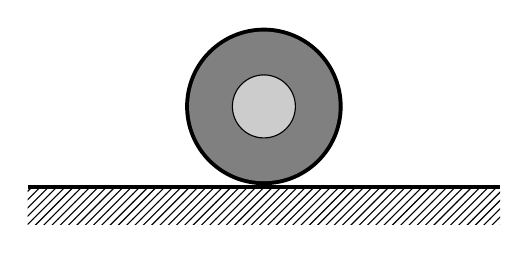
\begin{tikzpicture}
            \fill[black] (0,0) circle (1);
            \fill[black!50] (0,0) circle (.95);
            \draw[fill=black!20] (0,0) circle (0.4);
            \fill[black] (-3,-1) rectangle (3,-1.05);
            \fill[pattern=north east lines] 
              (-3,-1) rectangle (3,-1.5);
          \end{tikzpicture}
        }

        \tire
        \vs

      \part
        Draw the free-body diagram of the same point if the brakes have been applied and the car is slowing down without the tire skidding.

        \tire
        \vs

      \part
        Let's consider what happens to a car on an icy road.  
        
        If the car has a mass of about 1600~kg, then its weight (that is, force of gravity) is $mg \approx 16,000$~N.  That means, each of the four wheels must support a weight of about 4,000~N.

        The coefficients of friction between an average tire and and hard-packed snow on the road are $\mu_s \approx 0.20$ and $\mu_k \approx 0.15$.

        Let's say you have to slam on your brakes on hard-packed snow.  Calculate the amount of friction force the tire can provide if it doesn't slip.  Also, calculate the amount of friction force the tire can provide when it starts to slip.
        \vs[2]

      \part
        Cars with antilock brakes can sense when the tire starts to slip.  The brakes turn on and off rapidly to try to prevent the slipping.  Use your calculations above to explain why this is a good feature for a car.
        \vs 


    \end{parts}
    

\end{questions}

\end{document}